\subsection{Quality control after variant calling and genotype refinement}
After merging the datasets by recalling them, we carry out refinement with Beagle4 prior to phasing. We carry out a final QC prior to phasing. If SNP array data is available, we further check after genotype refinement with Beagle4 that the correlation between chip and sequence genotypes is greater than 0.95 for each sample (figure \ref{fig:adrp_refinement_chrom20_sample}).

\begin{figure}[htbp]
\centering
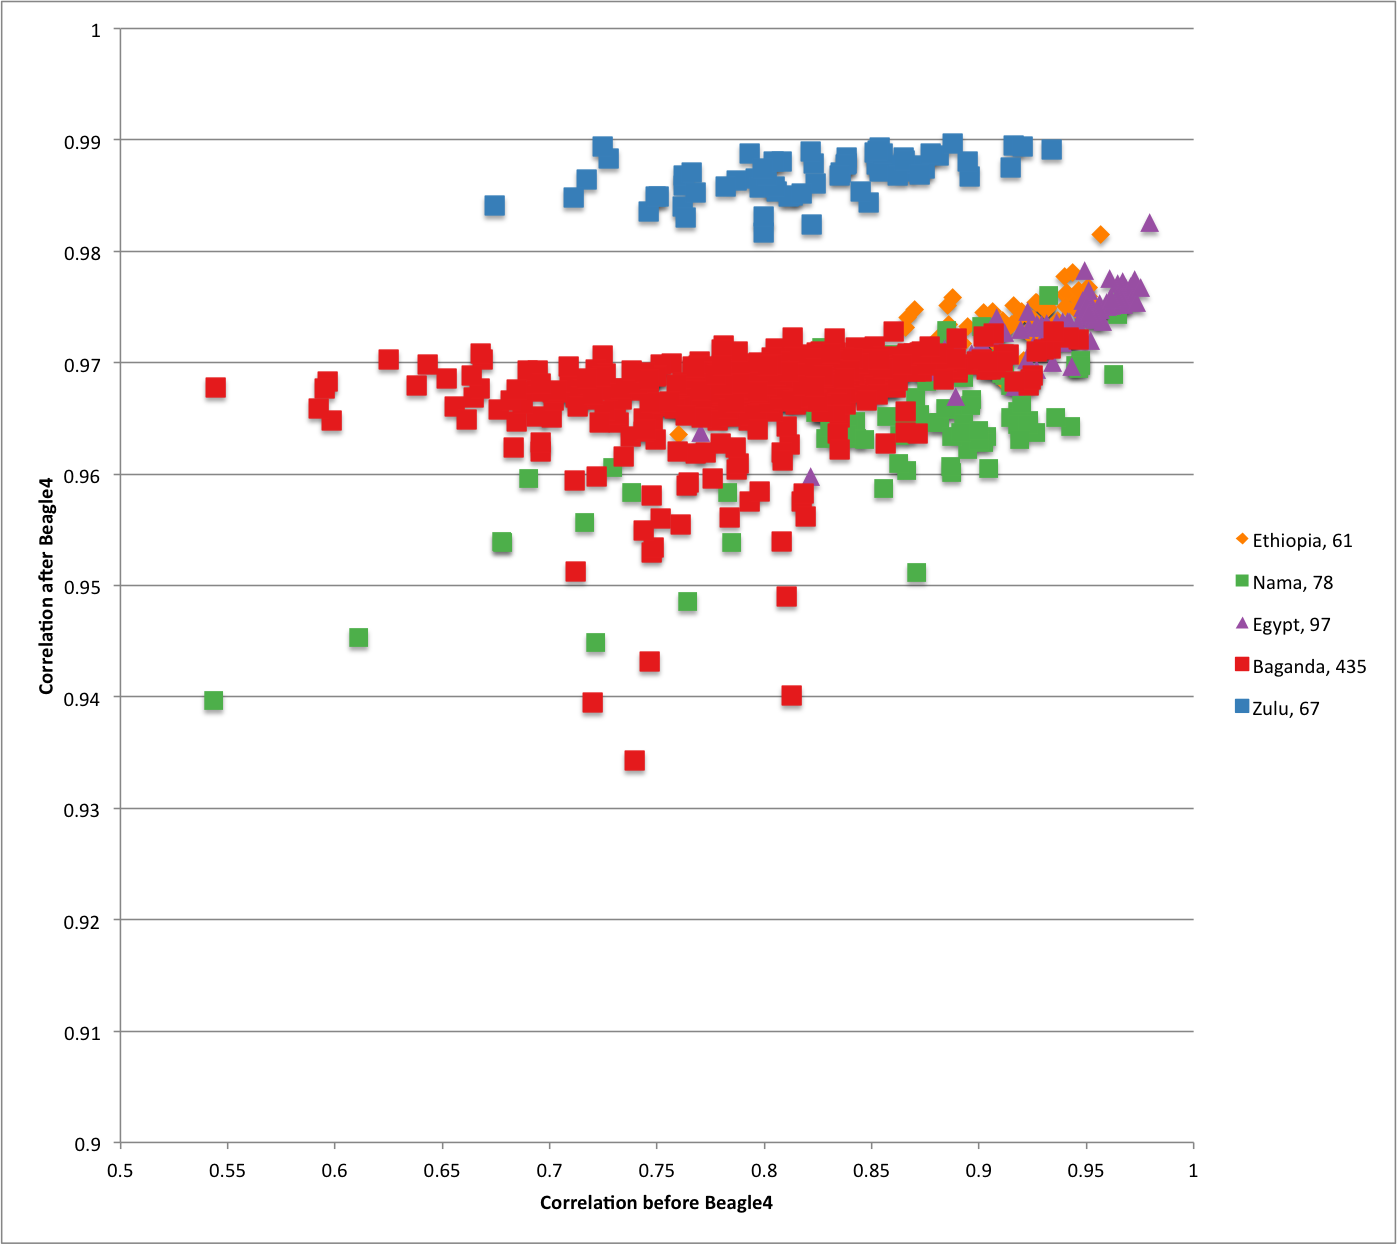
\includegraphics[width=0.8\textwidth]{adrp_refinement_chrom20_sample}
\caption{Correlation with SNP array genotypes on chromosome 20 before and after refinement of sequence data derived genotypes with Beagle4.}
\label{fig:adrp_refinement_chrom20_sample}
\end{figure}

We also check for heterozygosity outliers (\textgreater3SD per population) and PCA outliers after genotype refinement. Variant calling and genotype refinement is repeated if a sample either fails the check of genotype concordance, which is a sign of poor data quality, or fails the check of heterozygosity, which can be a sign of sample contamination or a population outlier.